\documentclass[12pt]{article}
\usepackage[margin=1in]{geometry}
\usepackage{amsmath}
\usepackage{amssymb}
\usepackage[tworuled, vlined, linesnumbered]{algorithm2e}
\usepackage[crop=pdfcrop,process=all,cleanup={.tex,.dvi,.ps,.pdf,.log}]{pstool}
\usepackage{enumitem}

\usepackage{amsthm}
\theoremstyle{definition}% upright text, extra space above and below
\newtheorem{definition}{Definition}[section]
\newtheorem{theorem}{Theorem}[section]
\newtheorem{corollary}{Corollary}[section]
\newtheorem{example}{Example}[section]
\newtheorem{lemma}{Lemma}[section]


%----------------------------------------------------------------------------------------
\title{University of Arizona Analytics Related to the COVID-19 Pandemic}
\author{ }

\date{} 

%----------------------------------------------------------------------------------------

\begin{document}
\maketitle
\section{Introduction}
This document describes/documents some of the analytics being conducted as a part of UA's COVID-19 response. 

\section{Flow of Funds}
These provide a high-level overview of the institutional flow of funds at UA.  $<$ More to come $>$

\subsection{Data Requirements}

\section{Program-related Opportunities}
We are interested in answering the following questions:
\begin{enumerate}
 \item What is the smallest set, $\alpha$, of courses that ``covers'' the largest number of degree requirements (i.e., courses) in the first two years of all undergraduate degree programs at UA?  (Note: this will probably contain a large number of general education courses.)
 \item What is the overlap of the set of online courses
\end{enumerate}

\begin{figure}
 \centerline{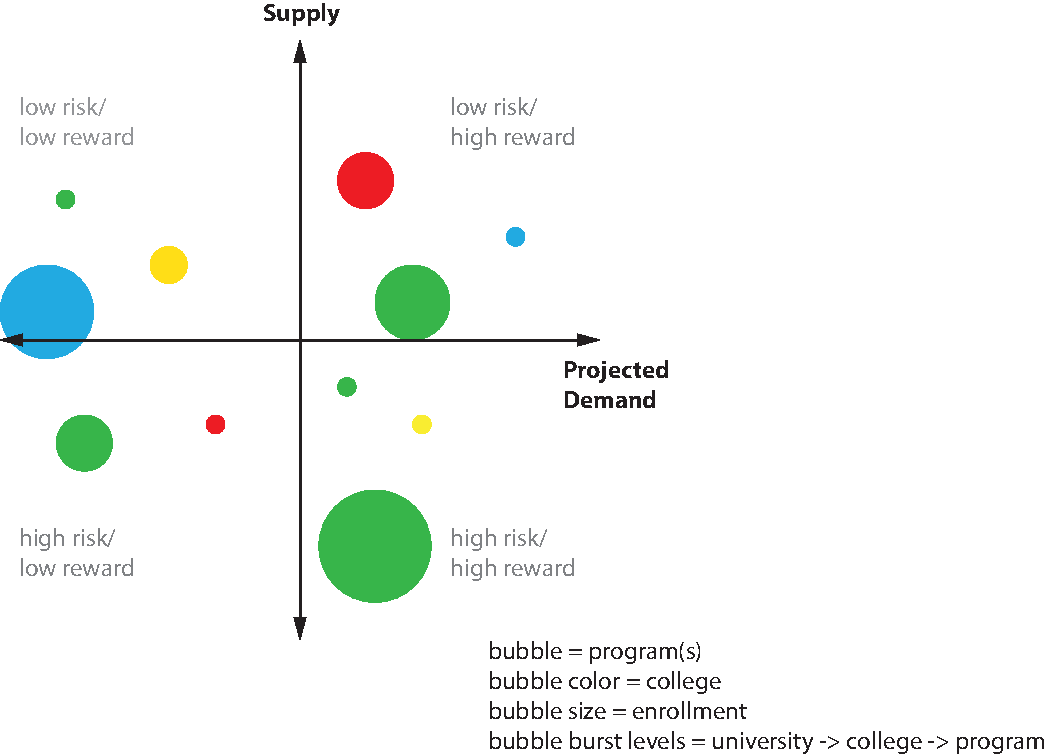
\includegraphics[width=4.75in]{./graphics/quad-bubble-supply-demand.pdf}}
 \caption{Supply and projected demand for the programs offered by the University of Arizona.}
\end{figure}

\begin{figure}
 \centerline{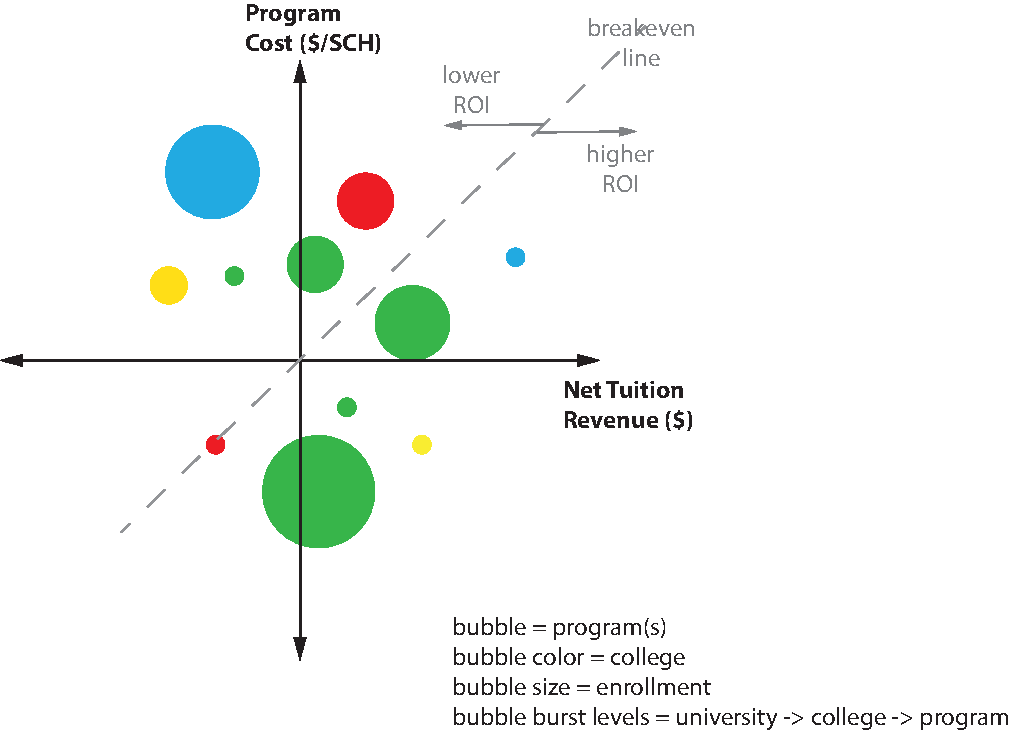
\includegraphics[width=4.75in]{./graphics/quad-bubble-ROI.pdf}}
  \caption{The return on investment (ROI) of the programs offered by the University of Arizona.}
\end{figure}


\subsection{Program Demand}
A number of these charts use program demand, projected program demand and projected program growth.  
In order to determine program demand, we used data made available through the U.S. Department of Labor's ONET website (\url{https://www.onetonline.org/}), where 
national and state-level wage and employment data and trends are provided.  This information is available according to the Classification of Instructional Programs (CIP) taxonomy.  For a given CIP code $x$,  we use $w(x)$ to denote the median annual wage for graduates from a program with CIP code $x$, and $n(x)$ is the number of people employed in professions related to CIP code $x$ in 2018.

the current demand associated with program $x$ using 2018 ONET data is denoted $\Alpha(x)$.

\subsection{Data Requirements}
 
\end{document}